%# -*- coding:utf-8 -*-
\chapter{血管模型中心线的提取}
\label{chap7}

\section{Introduction}
% no \PARstart
Cardiovascular diseases are among the most fatal illnesses worldwide \cite{WHO2013}.
The diseases occur when the stenosis or even blockages formed due to the build up of fatty substances on the inner wall of the blood vessels.
Percutaneous coronary intervention (PCI) is the gold standard in fighting the lethal diseases.
Due to its minimally-invasive nature, this procedure only causes small incision and much less trauma to the patients.
In addition, the hospitalization after the procedure is in turn dramatically shortened.
However, due to the very nature of minimally-invasiveness of PCI and the complex anatomic structure of the blood vessels, the learners need thorough and strict training before performing the procedure in action. %
What's worse, the practitioners in catheterization labs have to expose themselves under the ionizing radiation from the fluoroscope while examining the morphologies of the patients' vasculature. %

The surgical robotic systems for intravascular procedures have greatly changed this situation.
With the assistance of the robotic systems, cardiology practitioners need not to be worried about the radioactive exposure and the relative risks any more.
Like their ancestors (i.e., the traditional PCI procedure), the skills of manipulating the robotic system to do the surgery are also not easy for the junior residences and still require strict and sufficient training before applying the procedure on the real patients. %

The traditional ways of training PCI procedure are deeply rooted in the physical fashion, i.e., employing biological models (e.g. human cadavers and living animals) or non-biological models (e.g. phantoms). %
The former are disposable and ethic-disputed; let alone the tremendous expenditure on the preservation and feeding, and the distinction in anatomy between human and animal volunteer. %
The latter are stiff and lack of sufficient anatomic details, even though they can be used repeatedly.
Indeed, it is infeasible to conduct the training on the expensive robotic systems whilst ignoring the real needs in the catheterization labs.
To streamline the training and the practice of robotic PCI procedure, a well-designed computing simulation system is required.

The aim of our effort is to provide a training tool of convenience and effectiveness for the minimally-invasive intravascular robotic system \cite{Ji2011EMBC}.
In constructing this training vehicle, the anatomic structures in computing environment especially the vascular system are definitely one of the most substantial components.
The centerlines is an effective way of describing the shape of the model \cite{Ogniewicz1995}, which will provide accurate shape description for the path planning in interactive simulation.
In this paper, we developed an automatic approach based on the Voronoi diagram \cite{Antiga2003} to extract the centerlines of the vasculature.
The input of the proposed approach is the patient-specific image-based surface model of the vasculature, which is reconstructed by applying our previous work \cite{Yang2014ICRA}. %
Before computing the Voronoi diagram of the tubular surface model, several preprocessing should be performed.
First, the connectivity of the polygons that consisting the surface is validated thoroughly to include the largest connected polygons that is effective in representing the surface. %
Second, the bumpy and crusty surfaces are smoothed in order to reduce the effects on the computation of centerlines.
Third, the surfaces are subdivided to gain a more precise geometric feature.
Finally, the centerlines of the vessel model by solving the Eikonal equation in the fast marching flavor.
The capability of our approach in automatically extracting the centerlines of the vessel model is proved by the experimental results.

The rest of this paper is organized as follows.
Section II introduces the related work of the centerline extraction methods for three dimensional objects.
Section III outlines the work flow and describes the techniques used in this work.
Section IV describes the experiments, ending with a brief discussion.
The final section concludes the whole work.

\section{Related Work}

Many researches have been done since the earliest work on extracting the centerline was proposed by Blum \cite{Blum1967}.
According to reference \cite{Ogniewicz1995}, most of these methods fall into four categories: (1) topological thinning; (2) distance transformation; (3) ``prairie fire" approach; (4) Voronoi Diagram methods. %

Topological thinning methods \cite{Ma2002,Sadleir2002} implement the centerline extraction by iteratively remove most of the ``simple points" except the ones that are the end-points of the generated centerline models. %
By ``simple points", it means that the boundary points consisting the object such that their removals do not destroy the topology of the object.

Distance transformation methods \cite{Niblack1992} find the centerline by searching the local maximum among the minimal distances between the points interior of the shape and the boundary. %
However, they do not ensure the resulting centerlines are connected with each other.

``Prairie fire" methods \cite{Blum1967,Leymarie1992} compute the centerline by determining the intersection of the propagating interfaces with their sources located on the boundary of the shape. %

Voronoi diagram method \cite{Sherbrooke1996,Antiga2003} treats the centerline to be generated as a subset of the Voronoi diagram.
These methods are sensitive to the noises and the regularization of the boundary of the shape.

There are numbers of other methods that are not belong to any category listed above.
Ferchichi and Wang in \cite{Ferchichi2006} reported a clustering-based algorithm for centerline extraction both for 2D and 3D objects.
The algorithm was designed based on the idea of computing the maximal disks/balls determining the centerlines, which is achieved by executing the K-means algorithm iteratively on the object-points and their distance transforms. %
Egger \textit{et al.} \cite{Egger2007} reported a centerline extraction algorithm for the blood vessels using Dijkstra's shortest path algorithm, which was designed for the catheter simulation. %

\section{Methodologies}

This section discusses the design of the processing pipeline and details the principles of the consisting modules.
Before the actual centerline extraction begins, several processing aims to removing noises and smoothing the irregular surfaces need to be run to guarantee the quality of the input surface.
The image-based surface model of the blood vessels needs series of postprocessing steps depicted in Fig. \ref{fig:DataFlow} to meet the requirements of the centerline computing module. %
Among these processing steps, the first one is the validation of the connectivity of the consisting polygons.
During this process, the largest possible connected regions of the surface model are extracted.
Next, the surface smoothing step is needed to depress the ``crusts" and ``stairs" in the surface.
Then the normal vectors (i.e., normals) are computed to mark the ``inside" and the ``outside" of the surface model.
After that, the consisting polygons need to be subdivided under a specified criterion to facilitate the computation of the centerline extraction at the cost of longer computation time. %

%\subsection{Processing on Image-Based Surface Model}

\subsection{Connectivity Validation and Largest Region Extraction}

In this paper, the vasculature surface model is generated from the original medical volumetric data set by applying the approaches reported in our previous work \cite{Yang2014ICRA}. %
In order to find the largest region spanning the surface of the vasculature, the connectivity among the vertices in the image-based surface model needs to be thoroughly validated at the beginning of the processing. %
The inner working is to extract consisting polygons that share common vertices and meet some requirements.
In the present paper we implement the algorithm to extract the largest connected region from the input surface.
\begin{figure}[t]
\centering
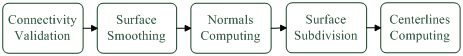
\includegraphics[width=3.2in]{Figures/DataFlow3.png}
\caption{Overview of the work flow.}
\label{fig:DataFlow}
\end{figure}

\subsection{Surface Smoothing and Normals Computing}

There are plenty of methods used for the surfaces smoothing in visualization.
To overcome the ``facets" by-produced during this approximation, an optimal surface smoothing algorithm treating this problem as low-pass filtering by extending Fourier analysis is adopted \cite{Taubin1996}. %
The adopted method is built upon the formulation of the \emph{discrete graph signals}, which means the functions based on directed graph.
The directed graph $G$ represents the polyhedral surfaces in this problem, which is denoted as the set $\left\{ 1, \ldots, n \right\}$ of nodes with a set of neighborhoods $\left\{ i^{\ast}: i = 1, \ldots, n \right\}$ of node $i$. %
A discrete graph signal can be represented as a vector $x = \left[ x_1, \ldots, x_n \right]^T$, where each component of the vector corresponds one node of the graph.
A polyhedral surface $S = \{ V, F \}$ of $n$ vertices can be treated as a directed graph, where the vertices $V$ corresponds the set of nodes $n$ and the faces $F$ the polygons formed by connected nodes. %

The discrete surface signal, the discrete graph signal defined on the associated graph, can be visualized as a piece-wise linear function defined on the surface.
The computation of the Discrete Fourier Transform (DFT) of the discrete surface signal defined on the surface is achieved by decomposing the surface signals as a linear combination of the eigenvectors of the Laplacian: %
\begin{equation}
\label{eqn:Laplacian}
\Delta x_i = \sum_{j \in i^{\ast}} w_{ij} \left( x_j - x_i \right),
\end{equation}
where $w_{ij}$ is the positive weight for each difference of $x_j - x_i$ and for a given vertex $i$, the sum of its weights are always one.
The matrix form of (\ref{eqn:Laplacian}) is
\begin{equation}
\label{eqn:LaplacianMatrix}
\Delta x = - K x,
\end{equation}
where $K = I - W$, with $I$ an identity matrix and $W$ the matrix of weights $w_{ij}$.

Choosing $0 \leq k_1 \leq \ldots \leq k_n \leq 2 $ as the eigenvalues of $K$, $r_1, \ldots, r_n$ the corresponding right eigenvectors, and $d_1, \ldots, d_n$ the associated dual basis of these eigenvectors, the above $K$ can be obtained as $K = \sum_{i} k_i r_i d_i^T$. %
%\begin{equation}
%\label{eqn:K}
%K = \sum_{i} k_i r_i d_i^T.
%\end{equation}
Thus there is a unique decomposition the discrete graph signal $x$, which can be obtained as a linear combination of the right eigenvectors $x = \sum_{i} \hat{x}_i r_i$, %$r_1, \ldots, r_n$
%\begin{equation}
%\label{eqn:x}
%x = \sum_{i} \hat{x}_i r_i,
%\end{equation}
where $\hat{x}_i = d_i^T x$ is the DFT of $x$.

According to signal processing theory, the filtering calculation on the signal $x$ is to change its frequency distribution at the reference of a transfer function $f$:
\begin{equation}
\bar{x} = \sum_{i} f(k_i) \hat{x}_i r_i = \left( \sum_{i} f(k_i) r_i d_i^T \right) x.
\end{equation}
The \emph{low-pass filtering} mechanism can be implemented by adjusting the weights in the following polynomial approximation
\begin{equation}
\label{eqn:Approximation}
f_{N}(k) = w_0 \frac{\theta}{\pi} T_0 (1 - k / 2) + w_n \sum_{n} \frac{2 \sin (n \theta)}{n \pi} T_n(1 - k / 2),
\end{equation}
where $\theta$ is the unique solution of $k = 2 (1 - \cos \theta)$ on $[0, \pi / 2]$, and $T$ the Chebyshev polynomial.
Here in this paper, the weights in (\ref{eqn:Approximation}) is adjusted to form a Hamming window, among sorts of them, which is demonstrated as follows:
\begin{equation}
\label{eqn:HammingWindow}
w_n = 0.54 + 0.46 \cos (n \pi / (N + 1) ).
\end{equation}

The normal vectors to the surfaces are computed after the surfaces are smoothed.

\subsection{Surface Subdivision}

A modified butterfly scheme for surface subdivision is used in order to refine the smoothed surface model \cite{Zorin1996}.
This scheme is designed in the flavor of interpolating and has been proved to be useful in the circumstances of subdivision for the complex especially irregular surfaces.
The ultimate goal is to improve the visualization of the input surface model without affecting its original shape.
The scalar value associated with the new vertex of the 2-dimensional triangulation is generated by calculating weighted sum of neighboring vertices using the proposed interpolation scheme. %
These vertices located in the neighborhood form the subdivision stencil, which determines the features of the scheme.
By analyzing the stencil, the scheme can quickly identify the relationship between the new vertex and the topology of its neighborhood.
The two most important cases in the surface are the regular sites and the extraordinary sites.
Once the initial subdivision cycles completed, the largest number of the vertices possessing the valence other than six is not exceeding one.
The new scalar value for the midpoint on each edge of the triangulation is calculated by the subdivision scheme falls into the following cases:
(1) edge connects two regular vertices;
(2) edge connects an extraordinary vertex and a regular vertex;
(3) edge connects two extraordinary vertices; and
(4) boundary edges.
%\begin{itemize}
%\item edge connects two regular vertices;
%\item edge connects an extraordinary vertex and a regular vertex;
%\item edge connects two extraordinary vertices;
%\item boundary edges.
%\end{itemize}
Among the above cases, only the first one belongs to the regular case, whilst the rest belong to the extraordinary case.

\subsection{Centerlines Extraction}

Centerlines, or medial axis, can be generally defined as the loci of the centers of the maximal inscribed disks (in 2D space) or spheres (in 3D space) inside an object.
Conversely, the envelop of all maximal inscribed disks/spheres is the boundary/surface of the object that contains these disks/spheres \cite{Amenta2001}.
Our approach employed the method demonstrated in \cite{Antiga2003}, which treats the centerlines as the minimal action paths on the Voronoi diagrams inside the model surface.
The Voronoi diagrams are the discrete approximation of the medial axis of the shape in two or three dimensional space.
The minimization of the line integral of the action path, which links two vertices in the Voronoi diagram, generates the center points that locally maximize their minimal distances to the boundary of the surface.
To do this, the method firstly computes the following Eikonal equation from a given starting point located on the Voronoi diagram
\begin{equation}
\label{eqn:Voronoi}
\left| \nabla T \right| = \frac{1}{R(u)},
\end{equation}
where $T$ marks the time of arrival, $R$ the radius of the maximal inscribed sphere at the time $T$, and $u$ the parametric space of the Voronoi diagram.
Then the centerline is obtained by calculating the following equation upon the previously demonstrated computation terminated:
\begin{equation}
\label{eqn:Centerlines}
\frac{dc}{ds} = - \nabla T,
\end{equation}
where $c$ denotes the centerlines, and $s$ the parametric space of $c$.
As a matter of fact, computation illustrated by (\ref{eqn:Centerlines}) is equivalent to finding the resulting centerline by applying the steepest descent method at each point on the Voronoi diagram.

\section{Experiments and Discussions}

\subsection{Data and Experimental Setup}

The vasculature surface models were generated by applying the approaches proposed in \cite{Yang2014ICRA} from the original CTA images acquired from some real patient.

In our experiments, the programs written in C++ ran on a desktop with Intel's 2.83GHz Core 2 Quad CPU and 4GB RAM.
%For the simplicity of description, part of the abdominal aorta is chopped off to serve as the sample data in our experiments described here (see Fig. \ref{fig:VOI}). %
Part of the abdominal aorta was chopped off to serve as the sample data in our experiments described here (see Fig. \ref{fig:VOI}). %
The approach can be applied straightly to the surface model of the whole abdominal aorta (see Fig. \ref{fig:OverlayGlobal}). %and Fig. \ref{fig:VisualizationModel}).
\begin{figure}[t]
\centering
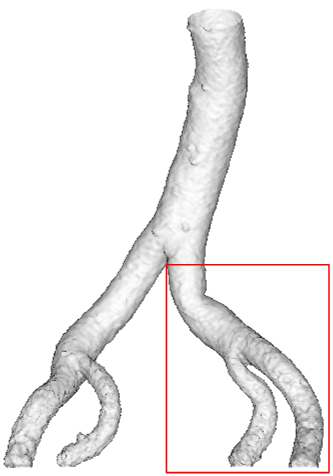
\includegraphics[height=2.4in]{Figures/VOI.png}
\caption{The original model surface (consists of $205,590$ polygons) and the VOI-extracted local part (in red square).}
\label{fig:VOI}
\end{figure}

%\subsection{Preprocessing for Centerline Extraction}

\subsection{Validating Connectivity of Image-Based Surface Model}

Before actually extracting the centerlines, the image-based surface model of the vasculature needs to be properly conditioned such that the computation can be operated successfully. %
The initial pass is the validation of the connectivity among the adjacent polygonal surfaces that consists of the whole visualization model.
The aim of this step is to find and connect the largest connected region in the given surface model (see Fig. \ref{fig:ConnectivityLocal}).
Table \ref{tbl:Connectivity} shows that the quantities of the consisting polygonal surfaces were not changed in local cases, whilst were decreased in global cases.
The former implies that the given (local) model was the largest connected region in the surface model before the validation.
The latter indicates that the largest connected region of the given model surface was fully extracted through the validation.
\begin{figure}[t]
\centering
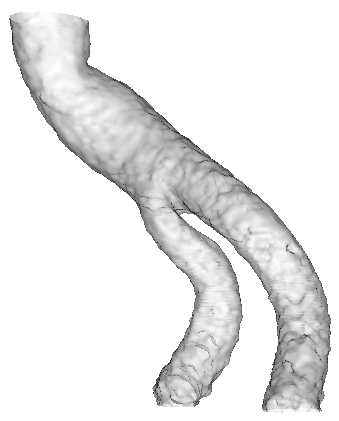
\includegraphics[width=1.5in]{Figures/connectivity_local.png}
\caption{Results of connectivity validation of model surface in local details (quantity of consisting polygons: $70,625$).}
\label{fig:ConnectivityLocal}
\end{figure}

\begin{table}[t]
\renewcommand{\arraystretch}{1.3}
\caption{Quantities of polygons before and after connectivity validation}
\label{tbl:Connectivity}
\centering
\begin{tabular}
{@{}llr@{}}
%{@{}llrr@{}}
\toprule
%\hline
%~      & ~                       & \multicolumn{2}{c}{Quantities} \\
%\cmidrule(4){3-4}
%~      & ~                       & Vertices & Polygons            \\
~      &                         & Quantities of polygons \\
%\midrule
\hline\hline
%Local  & Before validation       & N/A      & 70,625  \\
%~      & After validation        & N/A      & 70,625  \\
Local  & Before validation       & $70,625$  \\
~      & After validation        & $70,625$  \\
\hline\hline
%Global & Before validation       & N/A      & 205,590 \\
%~      & After validation        & N/A      & 205,452 \\
Global & Before validation       & $205,590$ \\
~      & After validation        & $205,452$ \\
\bottomrule
%\hline
\end{tabular}
\end{table}
\begin{figure}[t]
\centering
\subfloat{\includegraphics[width=1.5in]{Figures/smooth_30_1_local.png}%
\label{fig:Smooth30-1Local}}
\hfil
\subfloat{\includegraphics[width=1.45in]{Figures/smooth_30_01_local.png}%
\label{fig:Smooth30-01Local}}
\hfil
\subfloat{\includegraphics[width=1.5in]{Figures/smooth_100_1_local.png}%
\label{fig:Smooth100-1Local}}
\hfil
\subfloat{\includegraphics[width=1.45in]{Figures/smooth_100_01_local.png}%
\label{fig:Smooth100-01Local}}
\caption{Smoothing effects by applying different parameters: (a) $\text{pass band} = 0.1$, $\text{iterations} = 30$; (b) $\text{pass band} = 0.01$, $\text{iterations} = 30$; (c) $\text{pass band} = 0.1$, $\text{iterations} = 100$; (d) $\text{pass band} = 0.01$, $\text{iterations} = 100$.}%
\label{fig:SmoothLocal}
\end{figure}

%\begin{table}
%\renewcommand{\arraystretch}{1.3}
%\caption{Comparison of quantities of polygonal surfaces - Part I}
%\label{tbl:Eigenvalues}
%\centering
%\begin{tabular}{l||r}
%\hline
%\bfseries Connectivity validation & \bfseries Quantities \\
%\hline\hline
%Before                            & 757,538 \\
%After                             & 757,400 \\
%\hline
%\end{tabular}
%\end{table}

\subsection{Smoothing Connected Surface Model}

The centerline extracting method adopted in this work is sensitive to the noises on the input surface.
Due to the poor quality in some level of details of the original images, segmentation may introduce unnecessary uneven surfaces.
These artifacts in the surfaces can cause difficulties in the delivering of the virtual guidewires towards the hesion along the lumen of the model vessels.
To depress the noisy surface of the model, a surface smoothing module implemented based on low-pass filtering is applied.
There are two parameters associated with the smoothing module.
One of them specifies the number of iterations, which is equivalent to the degree of the polynomial approximating the windowed sinc function defined by (\ref{eqn:Approximation}).
The other determines the pass band of this low-pass filtering module.
Different sets of parameters were fed to the smoothing module in order to find the best results for the following processing (see Fig. \ref{fig:SmoothLocal}).
Observing these results, the parameters ($\text{pass band} = 0.01$, $\text{iterations} = 100$) used to generating the resulting surface in Fig. \ref{fig:Smooth100-01Local} demonstrated better effects than the rest.
%\begin{figure}[t]
%\centering
%\subfloat[]{\includegraphics[width=1.5in]{../Figures/smooth_30_1_local.eps}%
%\label{fig:Smooth30-1Local}}
%\hfil
%\subfloat[]{\includegraphics[width=1.45in]{../Figures/smooth_30_01_local.eps}%
%\label{fig:Smooth30-01Local}}
%\hfil
%\subfloat[]{\includegraphics[width=1.5in]{../Figures/smooth_100_1_local.eps}%
%\label{fig:Smooth100-1Local}}
%\hfil
%\subfloat[]{\includegraphics[width=1.45in]{../Figures/smooth_100_01_local.eps}%
%\label{fig:Smooth100-01Local}}
%\caption{Smoothing effects by applying different parameters: (a) $\text{pass band} = 0.1$, $\text{iterations} = 30$; (b) $\text{pass band} = 0.01$, $\text{iterations} = 30$; (c) $\text{pass band} = 0.1$, $\text{iterations} = 100$; (d) $\text{pass band} = 0.01$, $\text{iterations} = 100$.}%
%\label{fig:SmoothLocal}
%\end{figure}

\subsection{Subdivision Using Improved Butterfly Scheme}

To further attenuate the effects of noisy surfaces on extraction of centerlines and increase the precision of the centerlines extraction, the number of the polygons consisting the model surface has to be increased.
In order to achieve this, the smoothed surface need to be subdivided without introducing more perturbation.
Figure \ref{fig:SubdivisionLocal} illustrates that the subdivision computation based on the improved butterfly scheme.
At the same time, the quantities of the consisting polygonal surfaces increased substantially after the subdivision complete (see Table \ref{tbl:Subdivision}).
Comparing the quantities of the polygons before and after the subdivision in both cases, the quantities of the resulting polygons are about four times greater than the quantities of the input polygons due to the subdivision scheme employed in this work.
\begin{figure}[t]
\centering
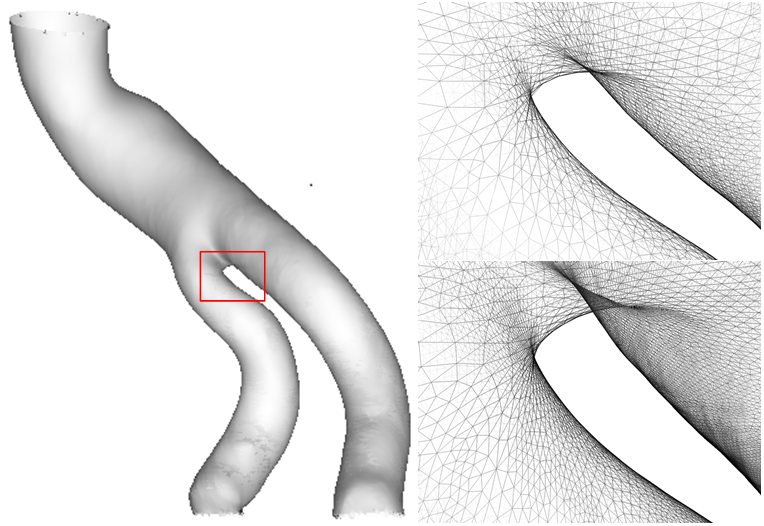
\includegraphics[width=3.0in]{Figures/subdivision.png}
\caption{Subdivision of smoothed surface by using improved butterfly scheme. \emph{Left}: subdivision in local details. \emph{Top right}: polyhedral surface before subdivision. \emph{Bottom right}: polyhedral surface after subdivision.}%
\label{fig:SubdivisionLocal}
\end{figure}

\begin{table}[t]
\renewcommand{\arraystretch}{1.3}
\caption{Quantities of polygons before and after subdivision using an improved butterfly scheme}
\label{tbl:Subdivision}
\centering
\begin{tabular}
%{@{}llr@{}}
{@{}llrr@{}}
\toprule
%\hline
%~      & ~                       & \multicolumn{2}{c}{Quantities} \\
%\cmidrule(4){3-4}
%~      & ~                       & Vertices & Polygons            \\
~      &                         & Quantities of polygons & Percentages ($\%$)\\
%\midrule
\hline\hline
%Local  & Before subdivision      & N/A      &  70,625  \\
%~      & After subdivision       & N/A      & 281,060  \\
Local  & Before subdivision      &  $70,625$  &\\
~      & After subdivision       & $281,060$  & 398 \\
\hline\hline
%Global & Before validation       & N/A      & 205,452  \\
%~      & After validation        & N/A      & 821,808  \\
Global & Before validation       & $205,452$  &\\
~      & After validation        & $821,808$  & 400 \\
\bottomrule
%\hline
\end{tabular}
\end{table}

%\begin{table}
%\renewcommand{\arraystretch}{1.3}
%\caption{Comparison of quantities of polygonal surfaces - Part II}
%\label{tbl:Eigenvalues}
%\centering
%\begin{tabular}{l||r}
%\hline
%\bfseries Subdivision  & \bfseries Quantities \\
%\hline\hline
%Before                 &  757,400 \\
%After                  & 3,029,600 \\
%\hline
%\end{tabular}
%\end{table}

\begin{figure}[t]
\centering
\subfloat{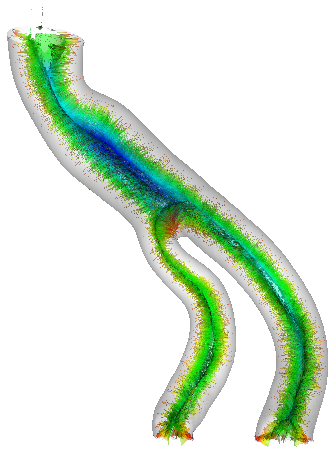
\includegraphics[width=1.5in]{Figures/overlay_100_01_voronoi_local.png}%
\label{fig:VoronoiLocal}}
\hfil
\subfloat{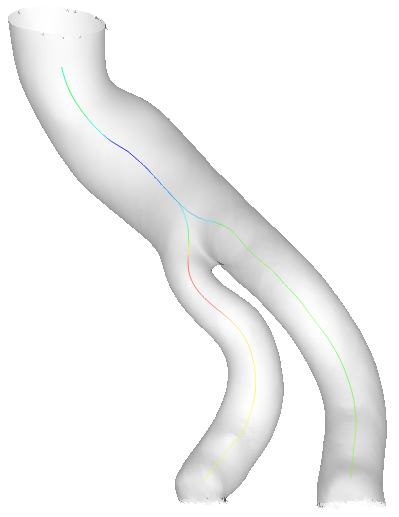
\includegraphics[width=1.5in]{Figures/overlay_100_01_centerlines_local.png}%
\label{fig:OverlayLocal}}
\caption{Centerlines extraction of the aorta in local details: (a) embedded Voronoi diagram; (b) centerlines inside the vessel.}%
\label{fig:CenterlinesLocal}
\end{figure}

\begin{figure}[t]
\centering
\subfloat{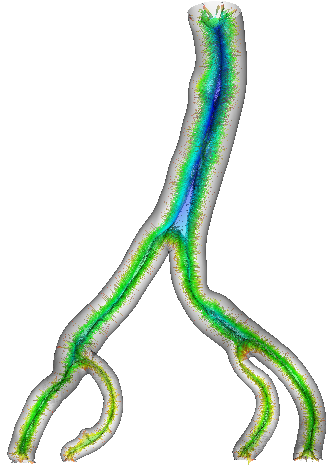
\includegraphics[height=2.0in]{Figures/overlay_100_01_voronoi.png}
%\caption{Voronoi diagrams of the abdominal aorta.}
\label{fig:VoronoiGlobal}}
\hfil
\subfloat{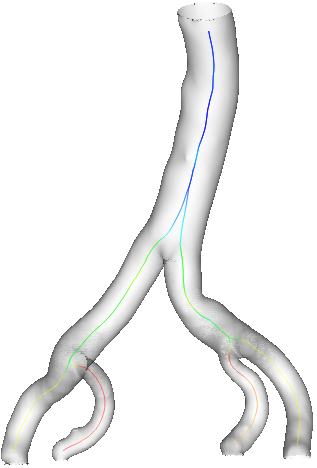
\includegraphics[height=2.0in]{Figures/overlay_100_01_centerlines.png}
%\caption{Centerlines of the abdominal aorta.}
\label{fig:OverlayGlobal}}
\caption{Centerlines extraction of the aorta in VOI. (a) Voronoi diagrams; (b) Centerlines. }
\label{fig:CenterlineGlobal}
\end{figure}

\subsection{Centerlines Extraction Based on Surface Model}

The centerlines extraction computation was performed on the subdivided surface model.
Firstly, the embedded Voronoi diagram of the preprocessed surface model is generated (see Fig. \ref{fig:VoronoiLocal}).
Secondly, the centerlines of the tubular surface model is computed (see Fig. \ref{fig:OverlayLocal}).
The colors marked on the Voronoi diagram and the centerlines denote the diameters of the local resection circle, decreasing from blue to red.
The same processing was straightly applied to the model surface of the whole abdominal aorta (see Fig. \ref{fig:VoronoiGlobal} and Fig. \ref{fig:OverlayGlobal}).
One can see from the details of the results that the starting and ending points are not exactly located at the ``entrances" or ``exits".
The reason of this is the Voronoi diagram on which the points consisting the centerlines exist never intersect with the model surface, i.e., the ending points of the centerlines are approaching the terminals of the surface model as near as possible, but never stick to them.
%\begin{figure}[t]
%\centering
%\subfloat[]{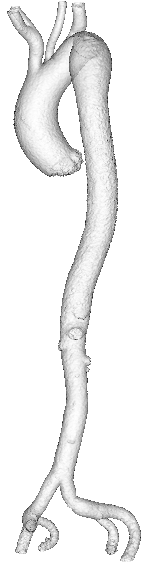
\includegraphics[width=0.7in]{../Figures/surface.eps}%
%\label{fig:SurfaceModel}}
%\hfil
%\subfloat[]{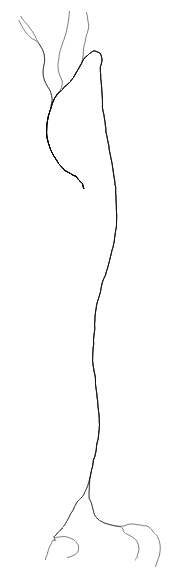
\includegraphics[width=0.9in]{../Figures/centerlines.eps}%
%\label{fig:CenterlinesModel}}
%\caption{Visualization models of the aorta: (a) image-based surface model (quantity of consisting polygons: $757,538$); (b) centerlines of the surface model.}%
%\label{fig:VisualizationModel}
%\end{figure}

\subsection{Discussions}

The computer programs used in this paper were written in C++ based on the Visualization Toolkit, an open source library aims at providing general facilities in the scientific visualization field \cite{Schroeder2000VTK}. %
To depress the unintended affections of the unstructured polygonal surfaces and the noises introduced by the image segmentation, series of steps were introduced in our experiments to extract the centerlines of the surface model of the vasculature. %
During this process, the quantities of the consisting polygons were obviously decreased for the extraction of the largest connected region in the surface model.
Due to the centerlines extraction computation is sensitive and expensive, we subdivided the smoothed surface model based on an improved butterfly scheme.
After this process, the quantities of the consisting polygonal surfaces were increased because of the refinement of the polygons.
With this step, the potential perturbation was further reduced, leading to much less errors which may occur during the computation of the centerlines extraction.
It is noteworthy that the extraction of centerlines for the model surface is an expensive computation both in time and space.
%The calculation of the whole aorta (see Fig. \ref{fig:VisualizationModel}) cost nearly eight hours on our desktop machine with dedicated modification on the code to fit the bulky data into the relatively limited memory. %
The calculation of the whole aorta cost nearly eight hours on our desktop machine with dedicated modification on the code to fit the bulky data into the relatively limited memory. %

\section{Conclusions and Future Work}
%The conclusion goes here.

Centerlines are useful in describing the shape of three dimensional objects.
In implementing the intravascular surgical simulation system, centerlines model of the vasculature will serve as the shape description for the simulation of path planning and navigation of the virtual guidewires/catheters.
In this paper, an automatic approach is designed and validated to extract the centerlines of the image-based patient-specific vasculature model.
The shape analysis presented here lays the foundation for our further research in visualizing the vessels that are closely related to the simulation of PCI procedure.

The connectivity of the polygons in the surface model is firstly checked to find out and remove the redundant polygons that are irrelevant to the actual surface.
Then the resulting surfaces are smoothed at the locations that seems to be uneven in order to prevent these perturbations against the centerlines computation.
After that, the surfaces are subdivided by applying an improved butterfly scheme with the aim of acquiring a more precise surface model.
Finally, the Eikonal equation of the time of arrivals of the embedded Voronoi diagram is computed to obtain the centerlines of the model surface.
Experiments are designed and carried out with the results in demonstrating the effectiveness of the developed approach.

In the future, our research directions are further optimization of the surface model on the one hand, and the visualization of other organs (e.g., heart) and the simulation of the typical phenomena (such as contrast injection, heart beat, etc.) during the procedure on the other. %
